\documentclass{beamer}
\usepackage{lipsum}
\usepackage[brazilian]{babel}
\usepackage[utf8]{inputenc}

\usepackage{enumerate}
\usepackage{dcolumn}
\usepackage{tabu}
\usepackage{colortbl}
\usepackage{booktabs}
\usepackage{changes}
\usepackage{listings}
\usepackage{placeins}
\usepackage{amsmath}

\usepackage{multirow}

\newcommand*{\Scale}[2][4]{\scalebox{#1}{$#2$}}%
\newcommand*{\Resize}[2]{\resizebox{#1}{!}{$#2$}}%

\usetheme[faculty=ppca,language=logo,framenumber,totalframenumber]{UniversiteitGent}

\title{Implantando uma arquitetura de serviços RESTful no CPD/UFSM}
\subtitle{ \textcolor{black}{Universidade Federal de Santa Maria} \\
			\textcolor{black}{\small{Centro de Processamento de Dados}} 
}



\author{Everton de Vargas Agilar (UnB / UFSM) \\
		Jader Adiel (UFSM)
}



\begin{document}

\begin{frame}
  \titlepage
\end{frame}




%%##################### PLANO #########################################

\section{Agenda}


\begin{frame}
  \frametitle{Agenda}

    \begin{itemize}

	    \item<1-> Barramento de serviços ERLANGMS
		    \begin{itemize}
		  	  \item<1->Objetivo do projeto
	    	  \item<1->Histórico do projeto
  	  	 	  \item<1->Design e princípios da arquitetura
  	  	 	  \item<1->Artigos produzidos para divulgar o barramento
		    \end{itemize}
	   	  \item<1-> 

	    \item<1-> Implantação do barramento no CPD/UFSM
		    \begin{itemize}
	        \item<1->Panorama geral sobre modernização
			\item<1->O que já foi feito
			\item<1->O que ainda precisa ser feito x prioridade
			\item<1->Principais desafios do trabalho
			\item<1->Caso prático 1: Web services implementados para o NCC
			\item<1->Caso prático 2: TClis do SIE invocando web services Java
		    \end{itemize}
   	    \item<1-> 
   	    


	 \end{itemize}	   	  

\end{frame}



%%##############################################################


\begin{frame}[c]{ }
\centering
\huge{Barramento de serviços ERLANGMS}
\end{frame}


\subsection{Objetivo do projeto}


\begin{frame}
\frametitle{Objetivo do projeto}

\begin{exampleblock}{ERLANGMS (https://github.com/erlangms)}
	
	É um projeto desenvolvido inicialmente na UnB para auxiliar na modernização de sistemas para uma arquitetura orientada a serviços 
	por meio de um barramento de serviços + SDK + processo 
	de modernização e arquitetura documentado (SMSOC).
	
\end{exampleblock}


\end{frame}





\begin{frame}

	\frametitle{Histórico do projeto}

	\centering
	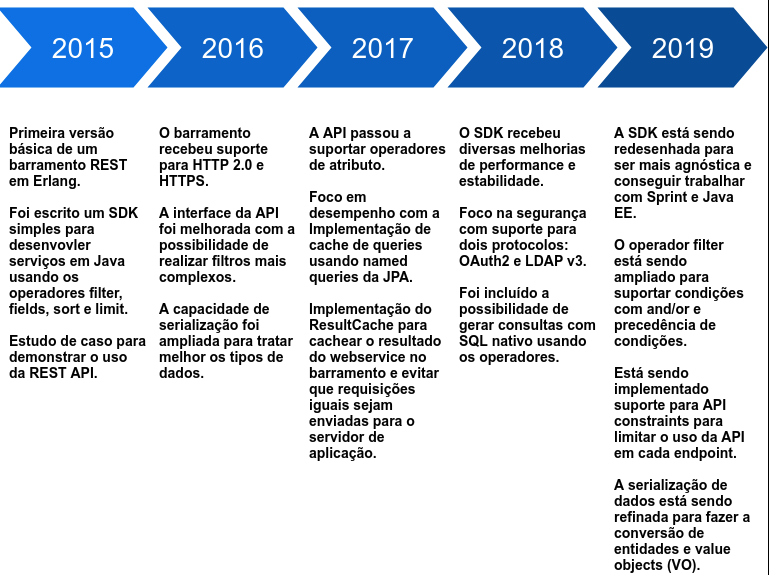
\includegraphics[scale=0.29]{img/historico.png}

\end{frame}



\begin{frame}
	\frametitle{Histórico do projeto \\ \small{Principais features em uso na UnB}}

\begin{exampleblock}{Features}
	
	\begin{itemize}
		\item<1->HTTP/2, HTTP/1.1, HTTPS (Secure TLS Listener);
		\item<1->LDAP v3 -- Proxy LDAP;
		\item<1->HTTP Basic authentication;
		\item<1->OAuth2 authentication;
		\item<1->SDK para criar serviços em Java;
		\item<1->Query Api -- filter, fields, sort, limit;
		\item<1->Suporte para Dados Abertos.
	\end{itemize}
	
\end{exampleblock}


\end{frame}




\begin{frame}
\frametitle{Design e princípios da arquitetura}

\begin{exampleblock}{Design e princípios da arquitetura}
	
	\begin{itemize}
		\item<1->Serviços especificados em catálogos de serviços;
		\item<1->Seguir as restrições RESTful quando possível;
		\item<1->Padrão \emph{Domain-Driven Design (DDD)} para modelagem do domnínio de negócio quando possível;
		\item<1->Ênfase em microserviços quando possível;
		\item<1->Baixa curva de aprendizado.
	\end{itemize}
	
\end{exampleblock}


\end{frame}


\begin{frame}
\frametitle{Artigos produzidos para divulgação do projeto}

\small{
	\begin{itemize}
		\item<1->A systematic mapping study on legacy system modernization -- 2016
		\item<1->Uma abordagem orientada a serviços para a modernização de sistemas legados -- 2016
		\item<1->Uma Implementação do Protocolo OAuth 2 em Erlang para uma Arquitetura Orientada a Serviço -- 2017
		\item<1->An experience report on the adoption of microservices in three brazilian government institutions -- 2018
		\item<1->Melhoria na Publicação de Dados Abertos: Automatização na Publicação e Indexação Semântica dos Dados -- 2018
		\item<1->Integração das Bases de Login e Senha dos Sistemas da Universidade de Brasília - UnB -- 2019
	\end{itemize}
}

\end{frame}



%%##############################################################







\section{Implantação do barramento na UFSM}


\begin{frame}[c]{ }
\centering
\huge{Implantação do barramento na UFSM}
\end{frame}


\begin{frame}
\frametitle{Panorama geral sobre modernização  \\ \small{Estudo realizado na UnB para identificar as estratégias de modernização}}

%% Mostra o diagrama de bolhas

\centering
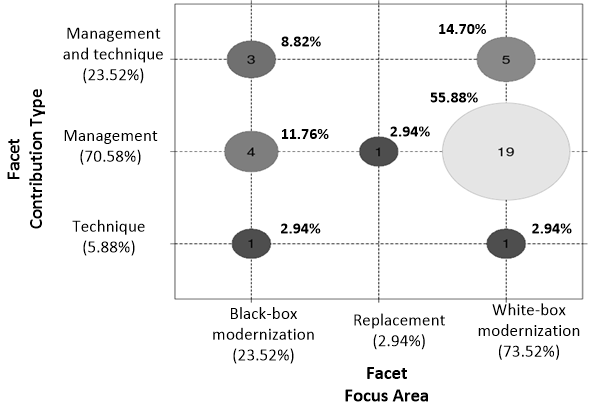
\includegraphics[scale=0.45]{img/bubble_diagram.png}

\end{frame}






\begin{frame}
\frametitle{O que já foi feito}

\begin{exampleblock}{O que já foi feito}
	
	\begin{itemize}
		\item<1->Implantação do barramento em partes, priorizando:
			\begin{itemize}
				\item<1->Query API
				\item<1->Subsistema de serialização;
				\item<1->Adaptar a interfaces do SDK para trabalhar de forma agnóstica com Java EE e Spring. 
			\end{itemize}
		\item<1->Features visando a migração de backends SIE para Java:
			\begin{itemize}
				\item<1->Suporte para serialização de dados como Dataset;
				\item<1->Provider RestApiMetaQueryProvider para migração de meta queries do Delphi;
				\item<1->Cliente REST implementado no Delphi com suporte a SSL.
			\end{itemize}
		
	\end{itemize}
	
\end{exampleblock}


\end{frame}

\begin{frame}
\frametitle{O que ainda precisa ser feito x prioridade}

\begin{exampleblock}{O que ainda precisa ser feito x prioridade}
	
	\begin{itemize}
		\item<1->Implementar o subsistema de autenticação/autorização OAuth2 (ou integrar por completo o barramento) -- Alto;
		\item<1->Analisar os principais métodos do TCliBusiness e prover um suporte adequado no SDK para facilitar a migração -- Alto;
		\item<1->Permitir gerar uma consulta por meio da Query API para buscar dados de um atributo lista de um objeto principal -- Baixo;
		\item<1->Permitir encadear funções nos atributos das entidades com o operador \% para modificar a forma como o dado é lido da fonte de dados -- Baixo.
		
		
	\end{itemize}
	
\end{exampleblock}







\end{frame}


\begin{frame}
\frametitle{Principais desafios do trabalho}

\begin{exampleblock}{Principais desafios do trabalho}
	\small{
	\begin{itemize}
		\item<1->Levando em consideração o custo de tempo para extrair as regras de negócios comuns automatizadas no core do SIE, estamos preferindo focar mais nas TClis dos frontends;
		\item<1->A quantidade de herança e, principalmente, métodos virtuais nas classes bases do pkCDESP tornam a migração mais demorada;
		\item<1->Há exceções, as meta-queries do Delphi podem ser convertidas facilmente em webservices como o SDK do barramento;
	\end{itemize}
}
\end{exampleblock}

\end{frame}




\begin{frame}
\frametitle{Principais desafios do trabalho}

\begin{exampleblock}{Principais desafios do trabalho}
\small{
	\begin{itemize}
		\item<1->Para o cliente REST do frontend Delphi obter os dados no formato Dataset para os TClis, é necessário especificar o schema dos dados. É relativamente fácil mas trabalhoso;
		\item<1->Pelo menos por enquanto, pelo fato do SIE CORE ser um artefato monolítico em termos de unidade de deploy, será bem mais desafiador o uso de microservices e Docker no futuro.
	\end{itemize}
}
\end{exampleblock}

\end{frame}


%%##############################################################


\begin{frame}
  \frametitle{Caso prático 1: Web services implementados para o NCC}

	\centering
	
\includegraphics[scale=0.4]{img/sdk.png}
  
\end{frame}


\begin{frame}
  \frametitle{Caso prático 2: TClis do SIE invocando web services Java}

	\centering
	
\includegraphics[scale=0.4]{img/sie.png}
  
\end{frame}






\begin{frame}[c]{ }
\centering
  \huge{Obrigado!}
\end{frame}


\end{document}



